\underline{Remarks}:
\begin{enumerate}[label={\arabic*)}]
	\item This is the formal solution of the linear system with constant coefficient. For big linear systems, this solution is difficult to obtain explicitely, since it involves an infinite number of matrix multiplications
	\item The homogeneous solution $x_n(t)$ depents on the set of initial conditions
		\begin{equation*}
			\vec{x}_0=\vec{x}(t_0);\quad \vec{x}_p \text{ depends only on the pertubation of }\vec{u}(t)
		\end{equation*}
	\item The answer of the system dpends on $\mat{H}=e^{\mat{A}t}$. If $\mat{H}(t)$ is given, we can calculate the time evolution for arbitrary pertubations of $\vec{u}(t)$ and 
\end{enumerate}
\underline{Example}: Linear system in 1D
\begin{align*}
	\dot{x}&=ax+u\\
	u(t)&=\begin{cases} 0 & t\leq 0 \\ u & t> 0 \end{cases};\qquad a\in\R \\
	\leadsto x(t)&=x_0e^{at}+\int\limits_0^tue^{a(t-\tau)}d\tau
\end{align*}
\textbf{\underline{\smash{Simple examples of non-linear systems}}}
\begin{enumerate}[label={(\roman*)}]
	\item The pendulum: The dynamics of the pendulum is described by the ordinary differential equation (ODE)
		\begin{equation*}
			\ddot{x}+\frac{g}{l}\sin(x)=0
		\end{equation*}
		We can rewrite the equation of 1st order ODEs:\vspace{-0.5 cm}
		\begin{multicols}{2}
			\begin{align*}
				\dot{x}_1 &= x_2\\
				\dot{x}_2 &= -\frac{g}{l}\sin(x_1)
			\end{align*}\columnbreak\\\\
			Obviously the rhs of the 2nd equation is non-linear and there fore the whole system.
		\end{multicols}
	\item The forced harmonic oszillatro:
		\begin{equation*}
			m\ddot{x}+b\dot{x}+kx=F\cos(t)
		\end{equation*}
		Again the ODE can be rewritten as a system of ODEs of first order:
		\begin{align*}
			\dot{x}_1&=x_2\\
			\dot{x}_2&=\frac{1}{m}\left(-kx_1-bx_2\right)+\frac{F}{m}\cos(x_3)\\
			\dot{x}_3&=1,\quad \text{ where } x_3=t
		\end{align*}
\end{enumerate}
The solution of a non-linear system is much more difficult than solving linear systems because linear systems often can be broken into parts.\\
In case of non-linear systems one often applies a geometric approach by using directly the properties of the system. This way, one might be able to construct the trajectories in phase space. 
\textbf{\underline{\smash{One-dimensional flow}}}\vspace{0.2 cm}\\
As an introductory example we consider the simple non-linear system $\dot{x}=\sin(x)$\\
This system can be solved analytically by seperation of variables:
\begin{align*}
	dt&=\frac{1}{\sin(x)}dx \underset{t_0=0}{\leadsto} t=\int\limits_{x_0}^{x}\frac{1}{\sin(x')}dx'\\
	\text{using} \int\frac{1}{\sin(x)}dx&=\ln\left|\frac{\sin(x)}{1+\cos(x)}\right|+c=\ln\left|\tan\left(\frac{x}{2}\right)\right|+c\\
	\leadsto t&=\ln\left|\frac{1+\cos(x_0)}{\sin(x_0)}\frac{\sin(x)}{1+\cos(x)}\right|
\end{align*}
The result is obviously difficult to interprete. By contrast, a graphical analysis of the system is simple.\\
We consider $\dot{x}=\sin(x)$ as a vector field on a line.
\begin{figure}[H]
	\begin{tikzpicture}
		\draw[->] (-3,0)--(3,0)node[below right]{$x$};
		\draw[->] (0,-2)--(0,2)node[above left]{$\dot{x}$};
		\draw (0.9,1.1)--(1,1)--(0.9,0.9);
		\draw (-0.9,-1.1)--(-1,-1)--(-0.9,-0.9);
		\draw[domain=-2.5:2.5,step=0.00001] plot(\x,{sin(90*\x)});
		\foreach \x \y in {-3/\frac{3}{2}\pi,-2/-\pi,-1/-\frac{\pi}{2},1/\frac{\pi}{2},2/\pi}{
			\draw (\x,0.1)--(\x,-0.1)node[below]{$\y$};
		}
		\draw[black,fill=white] (0,0)circle(2 pt);
		\draw[black,fill=black] (2,0)circle(2 pt)(-2,0)circle(2 pt);
	\end{tikzpicture}
\end{figure}
\noindent The flow is to the right, if $\dot{x}>0$ and to the left if $\dot{x}<0$. At points where $\dot{x}=0$ there is no flow.\\
$\leadsto \dot{x}=0$ corresponds to a fixed point.\\
\begin{figure}[H]
	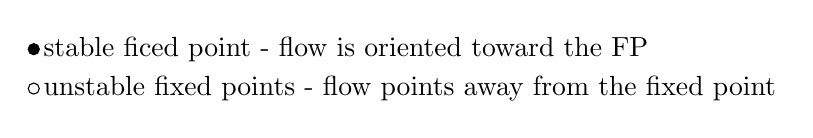
\begin{tikzpicture}
		\draw[fill=black] (0,0)circle(2 pt)node[right]{ stable ficed point - flow is oriented toward the FP};
		\draw[black,fill=white](0,-0.5)circle(2 pt)node[right]{ unstable fixed points - flow points away from the fixed point};
	\end{tikzpicture}
\end{figure}
\noindent Particle starting at $x=\frac{\pi}{4}$. The particle is moving to the right and will ultimately reach the FP at $x=\pi$.
\begin{figure}[H]
	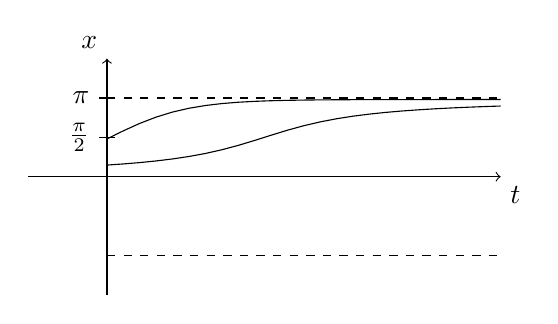
\begin{tikzpicture}
		\draw[->] (-1,0)--(5,0)node[below right]{$t$};
		\draw[->] (0,-1.5)--(0,1.5)node[above left]{$x$};
		\draw[dashed] (0,1)--(5,1)(0,-1)--(5,-1);
		\draw[domain=0:5,step=0.0001] plot(\x,{atan(\x-2)/180+0.5})plot(\x,{tanh(\x)/2+0.48});
		\draw (0.1,1)--(-0.1,1)node[left]{$\pi$};
		\draw (0.1,0.5)--(-0.1,0.5)node[left]{$\frac{\pi}{2}$};
	\end{tikzpicture}
\end{figure}
\noindent \textbf{\underline{\smash{Fixed points and stability}}}\vspace{0.2 cm}\\
We now generalize our system and consider $\dot{x}=f(x)$
Again, we get
\begin{figure}[H]
	\begin{tikzpicture}
		\draw[->] (-3,0)--(3,0)node[below right]{$x$};
		\draw[->] (0,-2)--(0,2)node[above left]{$\dot{x}$};
		\draw[domain=-2.5:2.5,step=1000] plot(\x,{0.3*(\x+1.5)*(\x-1.5)});
		\draw[black,fill=black] (-1.5,0)circle(2 pt);
		\draw[black,fill=white] (1.5,0)circle(2 pt);
	\end{tikzpicture}
\end{figure}
\noindent For the qualitative analysis of the trajectory. We consider x(t) as a "phase fluid", flowing with velocity \underline{\underline{$\dot{x}(t)=f(x(t))$}}\\
To find the solution $x(t)$, we place a particle at the phase point $x_0$ at $t=0$ and observe how it moves along the $x$-axis. This function is called trajectory. A picture showing all qualitatively ifferent trajectories is called phase portrait. FP represent stationary solutions, since we reach a FP $x^\ast$, where $f(x^\ast)=0$, $x(t)=x^\ast$ holds for all times.
\textbf{\underline{\smash{Example}}}: Find the FP of $f(x)=x^2-1$ and classify their stability:
\begin{equation*}
	x^\ast=-1 \text{ (stable)},\ x^\ast =1 \text{ (instable)}
\end{equation*}
\textbf{\underline{\smash{Population growths}}}:\vspace{0.2 cm}\\
Simplest model: $\dot{N}=rN$ $\leadsto N(t)=N_0e^{rt}$
\begin{itemize}
	\item[$\to$] unrestricted growth
\end{itemize}
More realistic: Finite resources have to be considered:
\begin{equation*}
	\dot{N}=rN\left(1-\frac{N}{k}\right)
\end{equation*}
\begin{figure}[H]
	\begin{multicols}{2}
		\begin{figure}[H]
			\begin{tikzpicture}
				\draw[->] (-0.5,0)--(3,0)node[below right]{$N$};
				\draw[->] (0,-1.5)--(0,1.5)node[above left]{$\dot{N}$};
				\draw[domain=0:2.5,step=0.001] plot(\x,{-\x*(\x-2)});
				\draw (1,0.1)--(1,-0.1)node[below]{$\frac{k}{2}$};
				\draw (2,0.1)--(2,-0.1)node[below]{$k$};
			\end{tikzpicture}
		\end{figure}\columnbreak
		\begin{figure}[H]
			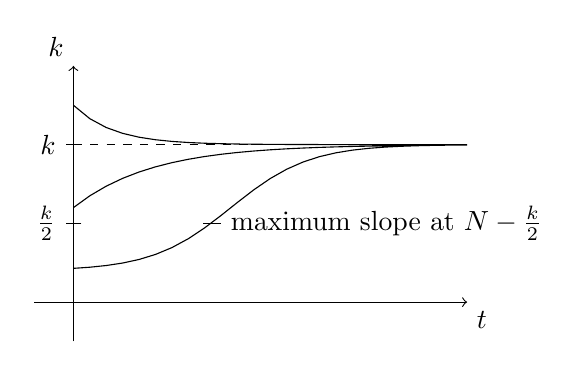
\begin{tikzpicture}
				\draw[->] (-0.5,0)--(5,0)node[below right]{$t$};
				\draw[->] (0,-0.5)--(0,3)node[above left]{$k$};
				\draw (0.1,2)--(-0.1,2)node[left]{$k$};
				\draw (0.1,1)--(-0.1,1)node[left]{$\frac{k}{2}$};
				\draw (1.65,1)--(1.875,1)node[right]{maximum slope at $N-\frac{k}{2}$};
				\draw[dashed] (0,2)--(5,2);
				\draw[domain=0:5,step=0.000001] plot(\x,{-0.8*exp(-\x)+2})plot(\x,{0.8*tanh(\x-2)+1.2})plot(\x,{0.5*exp(-2*\x)+2});
			\end{tikzpicture}
		\end{figure}
	\end{multicols}
\end{figure}
